\documentclass[10pt,a4paper]{article}
%\usepackage[utf8]{inputenc}
\usepackage{fontspec}
%\usepackage[polish]{babel}
\usepackage{amsmath}
%\usepackage{amsfonts}
%\usepackage{amssymb}
%\usepackage{makeidx}
%\usepackage{graphicx}
%\usepackage[left=2cm,right=2cm,top=2cm,bottom=2cm]{geometry}
\usepackage[colorlinks]{hyperref}
\usepackage{todonotes}
\usepackage{listings}
\usepackage{graphicx}

\usepackage{tikz}
\usepackage[europeanresistors,americaninductors]{circuitikz}



\author{Piotr Miedzik}
\title{MOSS}
\makeindex
\begin{document}
\maketitle

\listoftodos
\section{Projekt}


\begin{circuitikz}[american voltages]
\draw
(0,0) to [V, l_=$V_{in}$] (0,4)
      to [R=1k, l_=RB] (3,4)
      node[npn, anchor=B] (npn1) {}
      (npn1.E) node[npn, anchor=B] (npn2) {}
      (npn1.C) -- (npn2.C)
      (npn2.E) to [R, l_=$R_e$] 
      (4.75,0) 
      (npn1.C) to [short] (6,4.75)
      (6,0) to [V, l_=$V_{cc}$ ] (6,4.75)
      (6,0) -- (0,0);
      



%\begin{scope}[scale=0.8]
%\draw 
%  % rotor circuit
%  (0,0) to [short, *-] (6,0)
%  to [V, l_=$\mathrm{j}{\omega}_m \underline{\psi}^s_R$] (6,2) % rotor emf
%  to [R, l_=$R_R$] (6,4) % rotor resistance
%  to [short, i_=$\underline{i}^s_R$] (5,4) % rotor current

%  % stator circuit
%  (0,0) to [open, v^>=$\underline{u}^s_s$] (0,4) % stator voltage
%  to [short, *- ,i=$\underline{i}^s_s$] (1,4) % stator current
%  to [R, l=$R_s$] (3,4) % stator resistance
%  to [L, l=$L_{\sigma}$] (5,4) % leakage inductance
%  to [short, i_=$\underline{i}^s_M$] (5,3) % magnetizing current
%  to [L, l_=$L_M$] (5,0); % magnetizing inductance



	   
%      (npn.E) node[below=2mm] {C} % Collector (of the (whole) IGBT)
%      (npn.B) node[left=7mm] {npn};
%
%      (0,7) to[R,l_=$R_B$] (0,5) -- (pnp.C) % body region spreading resistance%

%      (0,7) -- (5,7)

%      to[Tnigfete,n=mosfet] (5,5) % MOSFET
%      to[Tnjfet,n=jfet,mirror] (5,3) % JFET
%      to[R,l=$R_{\text{mod}}$] (5,1) % drift region resistance (modulated)
%      -- (pnp.B)

%      (mosfet.G) node[anchor=west] {G} % Gate
%      (mosfet.B) node[anchor=east] {MOSFET}
%      (jfet) node[anchor=west] {JFET}

%      (2,7) -- (2,6) to[Tnpn,n=npn,mirror] (2,4) -- (2,1)
%      (npn.B) -- (0,5)
%      (npn.B) node[right=7mm] {npn}

%      (3,7.5) to[short,n=IGBTE] (3,7) % Emitter
%      (IGBTE) node[above=2mm] {E};
%\end{scope}
% Symbol with voltage and current:
%\draw (8,3) node[nigbt] (igbt) {}
%      (igbt.C) node[anchor=east] {C} % Collector
%      (igbt.B) node[anchor=east] {G} % Gate
%      (igbt.E) node[anchor=east] {E} % Emitter

%      (igbt.C) to [short, i<_=$I_C$] +(0,+5mm) %current
%      (igbt.C) to [open, v^>=$U_{CE}$] (igbt.E) -- +(0,-2mm); %voltage

\end{circuitikz}
\todo[inline]{Poprawić obrazek}

\begin{align}
V_{in} = 
\begin{cases} 
1.5V, & \mbox{OP}\\
1, & \mbox{AC}
\end{cases}
\end{align}


\begin{circuitikz}[american voltages,american currents]
\draw
(0,0) to [V, l_=$V_{in}$] (0,8) 
      to [R=1k, l_=$RB_{15}$] (2,8)
      to [R=1k, l_=$R_{B53}$] (4,8)
      to [cI=$i_{B73}$, *-] (4,6) 
      to [short, -*] (6,6)
(4,8) to [short, *-*] (6,8)
      to [C=$c_{73}$,*-*] (6,6)
(6,8) to [C=$c_{72}$, *-*] (8,8)
      to [cI=$i_{C23}$, *-] (8,6) 
      to [short, -*] (6,6)
(4,6) to [short, *-] (4,4)
	  to [R=$R_{B36}$] (6,4)
	  to [cI=$i_{B64}$, *-] (6,2)
	  to [short, -*] (8,2)
(6,4) to [short, *-*] (8,4)
      to [C=$c_{64}$, *-*] (8,2)
(8,4) to [C=$c_{62}$, *-*] (10,4)
      to [cI=$i_{C24}$, *-] (10,2)
      to [short, -*] (8,2)
      to [R=$R_{e40}$] (8,0)
(10,4) to [short, *-*] (10,8)
(12,0) to [V, l_=$V_{cc}$ ] (12,8)
      to [short, -*] (8,8)
(12,0) -- (0,0);
\end{circuitikz}



\todo[inline]{Wstawić schematy zastępcze}
\subsection{Parametry tranzystora}

\[
i_B = \frac{I_S}{BF} \left( exp \left(\frac{u_{BE}}{NFU_T} \right) - 1 \right) +
\frac{I_S}{BR} \left( exp \left(\frac{u_{BC}}{NRU_T} \right) - 1 \right)
\]
\[
i_C = I_S \left( exp \left(\frac{u_{BE}}{NFU_T} \right) - exp \left(\frac{u_{BC}}{NRU_T} \right) \right) -
\frac{I_S}{BR} \left( exp \left(\frac{u_{BC}}{NRU_T} \right) - 1 \right)
\]
\[
C_{BE} = \frac{TF\left( 1 + \frac{1}{BF} \right)I_S}{NFU_T} exp \left(\frac{u_{BE}}{NFU_T} \right) +
\frac{C_{jE0}}{{\left( 1 - \frac{\u_{BE}}{VJE} \right)}^{MJE}}
\]
\[
C_{BC} = TR \frac{I_S}{NRU_T} exp \left(\frac{u_{BC}}{NRU_T} \right) +
\frac{C_{jC0}}{{\left( 1 - \frac{\u_{BC}}{VJC} \right)}^{MJC}}
\]

\todo{Dodać parametry tranzystora podane przez prowadzącego}

\section{Analiza OP}
\subsection{Schemat zastępczy dla analizy OP}
\begin{circuitikz}[american voltages,american currents]
\draw
(0,0) to [V, l_=$E_{10}$] (0,8)
      to [R=1k, l_=$RB_{15}$] (2,8)
      to [R=1k, l_=$R_{B57}$] (4,8)
      to [cI=$i_{B73}$, *-] (4,6) 
      to [short, -*] (6,6)
(4,8) to [short, *-*] (6,8)
(8,8)
      to [cI=$i_{C23}$, *-] (8,6) 
      to [short, -*] (6,6)
(4,6) to [short, *-*] (4,4)
	  to [R=$R_{B36}$] (6,4)
	  to [cI=$i_{B64}$, *-] (6,2)
	  to [short, -*] (8,2)
(6,4) to [short, *-*] (8,4)
(10,4)
      to [cI=$i_{C24}$, *-] (10,2)
      to [short, -*] (8,2)
      to [R=$R_{e40}$] (8,0)
(10,4) to [short, *-*] (10,8)
(12,0) to [V, l_=$E_{20}$ ] (12,8)
      to [short, -*] (8,8)
(12,0) -- (0,0);
\end{circuitikz}
\todo[inline]{Wstawić schemat}

\[
E_{10} = 1.5V
\]
\[
E_{20} = 12V
\]
\[
G_{15} = \frac{1}{RB}
\]
\[
G_{57} = \frac{1}{R_{B57}}
\]
\[
G_{36} = \frac{1}{R_{B36}}
\]
\[
G_{40} = \frac{1}{R_{e40}}
\]

Dla gałęzi ic:
\[
i_{23}^{(p+1)}= g_{be23}^{(p)} \left( v_7^{(p+1)} - v_3^{(p+1)} \right) +
 g_{bc23}^{(p)} \left( v_7^{(p+1)} - v_2^{(p+1)} \right) + j_{23}^{(p)}
\]
\[
g_{be23}^{(p)} = \frac{I_S}{NF \cdot U_T} \cdot exp \left( \frac{v_7^{(p)} - v_3^{(p)}}{NF \cdot U_T} \right)
\]
\[
g_{bc23}^{(p)} = 
- \frac{I_S}{NR \cdot U_T} \cdot exp \left( \frac{v_7^{(p)} - v_2^{(p)}}{NR \cdot U_T} \right)
- \frac{I_S}{BR \cdot NR \cdot U_T} \cdot exp \left( \frac{v_7^{(p)} - v_2^{(p)}}{NR \cdot U_T} \right)
\]

\[
j_{23}^{(p)} = I_S \left( exp \left(  \frac{v_7^{(p)} - v_3^{(p)}}{NF \cdot U_T} \right) 
-exp \left( \frac{v_7^{(p)} - v_2^{(p)}}{NR \cdot U_T} \right)
\right) -
\frac{I_S}{BR} \left( exp \left( \frac{v_7^{(p)} - v_2^{(p)}}{NR \cdot U_T} \right) - 1 \right) - g_{be23}^{(p)} \left( v_7^{(p)} - v_3^{(p)} \right) -
g_{bc23}^{(p)} \left(v_7^{(p)} -v_2^{(p)} \right)
\]
Dla gałęzi ib
\[
i_{73}^{(p+1)}= g_{be73}^{(p)} \left( v_7^{(p+1)} - v_3^{(p+1)} \right) +
 g_{bc73}^{(p)} \left( v_7^{(p+1)} - v_2^{(p+1)} \right) + j_{73}^{(p)}
\]
\[
g_{be73}^{(p)} = \frac{I_S}{BF \cdot NF \cdot U_T} \cdot exp \left( \frac{v_7^{(p)} - v_3^{(p)}}{NF \cdot U_T} \right)
\]
\[
G_{bc73}^{(p)} = 
- \frac{I_S}{BR \cdot NR \cdot U_T} \cdot exp \left( \frac{v_7^{(p)} - v_2^{(p)}}{NR \cdot U_T} \right)
\]

\[
j_{73}^{(p)} = \frac{I_S}{BF} \left( exp \left(  \frac{v_7^{(p)} - v_3^{(p)}}{NF \cdot U_T} \right) 
- 1 \right) +
\frac{I_S}{BR} \left( exp \left( \frac{v_7^{(p)} - v_2^{(p)}}{NR \cdot U_T} \right) - 1 \right) -
g_{be73}^{(p)} \left( v_7^{(p)} - v_3^{(p)} \right) -
G_{bc73}^{(p)} \left(v_7^{(p)} -v_2^{(p)} \right)
\]

\todo[inline]{Powielić dla drugiego NPN}

\subsection{Wyniki symulacji LT Spice}

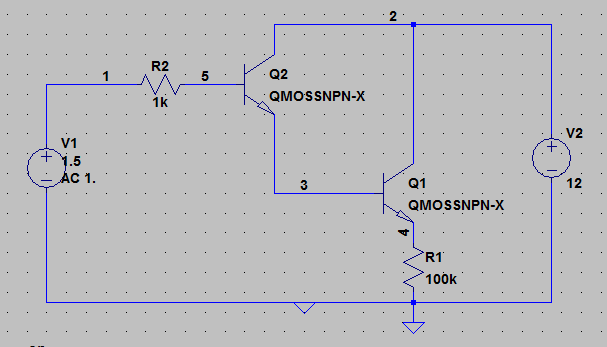
\includegraphics{schemat.png}

\begin{lstlisting}
       --- Operating Point ---

V(2):	 12	 voltage
V(5):	 1.49996	 voltage
V(3):	 1.00103	 voltage
V(4):	 0.432637	 voltage
V(1):	 1.5	 voltage
Ic(Q1):	 4.01568e-006	 device_current
Ib(Q1):	 3.10684e-007	 device_current
Ie(Q1):	 -4.32637e-006	 device_current
Ic(Q2):	 2.72276e-007	 device_current
Ib(Q2):	 3.84079e-008	 device_current
Ie(Q2):	 -3.10686e-007	 device_current
I(R2):	 -3.84079e-008	 device_current
I(R1):	 4.32637e-006	 device_current
I(V2):	 -4.28796e-006	 device_current
I(V1):	 -3.84079e-008	 device_current
\end{lstlisting}

\subsection{Wyniki symulacji Matlab}
\section{Analiza AC}
\end{document}